% CVPR Paper Template; see https://github.com/cvpr-org/author-kit
\documentclass[10pt,twocolumn,letterpaper]{article}

%%%%%%%%% PAPER TYPE  - PLEASE UPDATE FOR FINAL VERSION
% \usepackage{cvpr}              % To produce the CAMERA-READY version
\usepackage[review]{cvpr}      % To produce the REVIEW version
% \usepackage[pagenumbers]{cvpr} % To force page numbers, e.g. for an arXiv version

%% This file contains a number of tweaks that are typically applied to the main document.
%% They are not enabled by default, but can be enabled by uncommenting the relevant lines.


%%
%% Official support for 2-column teaser figure
%%
\usepackage{cuted} %< for strip environment

%%
%% For auto-referencing of figures (see fig/teaser.tex and \label{} therein) 
%%
\usepackage{currfile} %< for \currfilebase macro

%%
%% caption and (global) spacing overrides
%%
\usepackage{caption} %< for "\captionof" commands (teaser)
% \setlength{\abovecaptionskip}{.5em} % space above caption
% \setlength{\belowcaptionskip}{1em} % space below caption

%%
%% Inline annotations; for predefined colors, refer to "dvipsnames" in the xcolor package:
%% https://tinyurl.com/overleaf-colors
%%
\newcommand{\red}[1]{{\color{red}#1}}
\newcommand{\todo}[1]{{\color{red}#1}}
\newcommand{\TODO}[1]{\textbf{\color{red}[TODO: #1]}}
%%
%% Disable for camera ready / submission by uncommenting these lines:
%%
% \renewcommand{\TODO}[1]{}
% \renewcommand{\todo}[1]{#1}

%%
%% Work harder in optimizing text layout. Typically shrinks text by 1/6 of page, enable
%% it at the very end of the writing process, when you are just above the page limit.
%%
% \usepackage{microtype}

%%
%% Fine-tune paragraph spacing.
%%
% \renewcommand{\paragraph}[1]{\vspace{.5em}\noindent\textbf{#1.}}

%%
%% Globally adjusts space between figure and caption.
%%
% \setlength{\abovecaptionskip}{.5em}

%%
%% Allows "the use of \paper to refer to the project name"
%% with automatic management of space at the end of the word.
%%
% \usepackage{xspace}
% \newcommand{\paper}{ProjectName\xspace}

%%
%% Commonly used math definitions.
%%
% \DeclareMathOperator*{\argmin}{arg\,min}
% \DeclareMathOperator*{\argmax}{arg\,max}

%%
%% Tighten underline.
%%
% \usepackage{soul}
% \setuldepth{foobar}

%%
%% Reconfigure paragraph (tweaks spacing)
%%

\usepackage{multirow}
\usepackage{amsfonts}

\definecolor{cvprblue}{rgb}{0.21,0.49,0.74}
\usepackage[pagebackref,breaklinks,colorlinks,allcolors=cvprblue]{hyperref}

%%%%%%%%% PAPER ID  - PLEASE UPDATE
\def\paperID{*****} % *** Enter the Paper ID here
\def\confName{CVPR}
\def\confYear{2027}

% float/caption spacing (margins and fonts untouched)
\setlength{\textfloatsep}{8pt plus 2pt minus 2pt}
\setlength{\floatsep}{6pt plus 2pt minus 2pt}
\setlength{\intextsep}{6pt plus 2pt minus 2pt}
\setlength{\dbltextfloatsep}{8pt plus 2pt minus 2pt}
\setlength{\abovecaptionskip}{4pt}
\setlength{\belowcaptionskip}{2pt}

\newcommand{\bridge}{\textsc{Bridge}}
\newcommand{\medforge}{\textsc{MedForge}}
\newcommand{\medforgepp}{\textsc{MedForge++}}

\title{MedForge++: Bridging Reinforcement Learning for Generalizable\\Medical Forgery Detection Across Organ Domains}

\author{Anonymous CVPR submission}

\begin{document}
\maketitle
\begin{abstract}
Text-guided medical image editing models can now generate realistic medical forgeries by inserting or removing lesions from authentic scans, posing new challenges for trustworthy AI-assisted diagnosis. Existing benchmarks cover only a few organ domains, making generalization across clinical settings difficult to evaluate. We introduce \medforgepp{}, a large-scale benchmark that extends existing medical forgery datasets with 7{,}800 newly annotated kidney CT and colon polyp images, for 103{,}076 images spanning multiple modalities, organ systems, and forgery types. Building on this benchmark, we introduce \bridge{}, a Qwen3-VL-8B detector trained in three stages: failure-targeted replay supervised fine-tuning, forgery-aware reinforcement learning, and training-free cross-stage LoRA weight interpolation. \bridge{} reaches 96.96\% accuracy and 96.18\% macro-F1 on the Cross-Forgery benchmark, outperforming the best previously reported results. On the full \medforgepp{} corpus, a domain-routed deployment of \bridge{} reaches 93.86\% accuracy and 93.49\% macro-F1, surpassing the publicly released \medforge{}-Reasoner (89.85\%/89.05\%). We provide the first systematic evaluation of a publicly released medical forgery detector on previously unseen organ domains, and release our benchmark, training pipeline, and evaluation protocols.
\end{abstract}

\section{Introduction}
\label{sec:intro}
Diffusion models and multimodal foundation models now let a user edit an image simply by describing the change \cite{diffusion_survey_2024, latent_diffusion_2022, instruct_pix2pix_2023, multimodal_foundation_models_2023}. These capabilities have rapidly extended to medical imaging: text-guided editors can insert or remove a lesion from a scan using only a short prompt \cite{text_guided_medical_editing_2025, medisyn_2024, miedb_2026, m3dsynth_2023}. Built for legitimate uses such as augmentation and privacy-preserving synthesis \cite{medical_data_augmentation_2023, synthetic_medical_data_2024}, the same models can fabricate convincing medical evidence, and \medforge{} \cite{medforge2026} recently showed this is not hypothetical for chest X-ray, brain MRI, and fundus photography. The risks differ from a manipulated photograph: an implanted or removed lesion can directly change a diagnosis, since clinicians reason from the image itself, and the CT-GAN attack already showed a conditional GAN can inject or remove lung lesions convincingly enough to fool automated classifiers and radiologists \cite{ctgan_attack_2019}. A tampered scan can also corrupt a medical record \cite{medical_record_integrity_2018} or undermine a clinical study's reproducibility \cite{scientific_integrity_imaging_2026}. Each harm depends on the same property: a small, localized, anatomically plausible edit a human is unlikely to notice without forensic tools.
\begin{figure}[t]
\centering
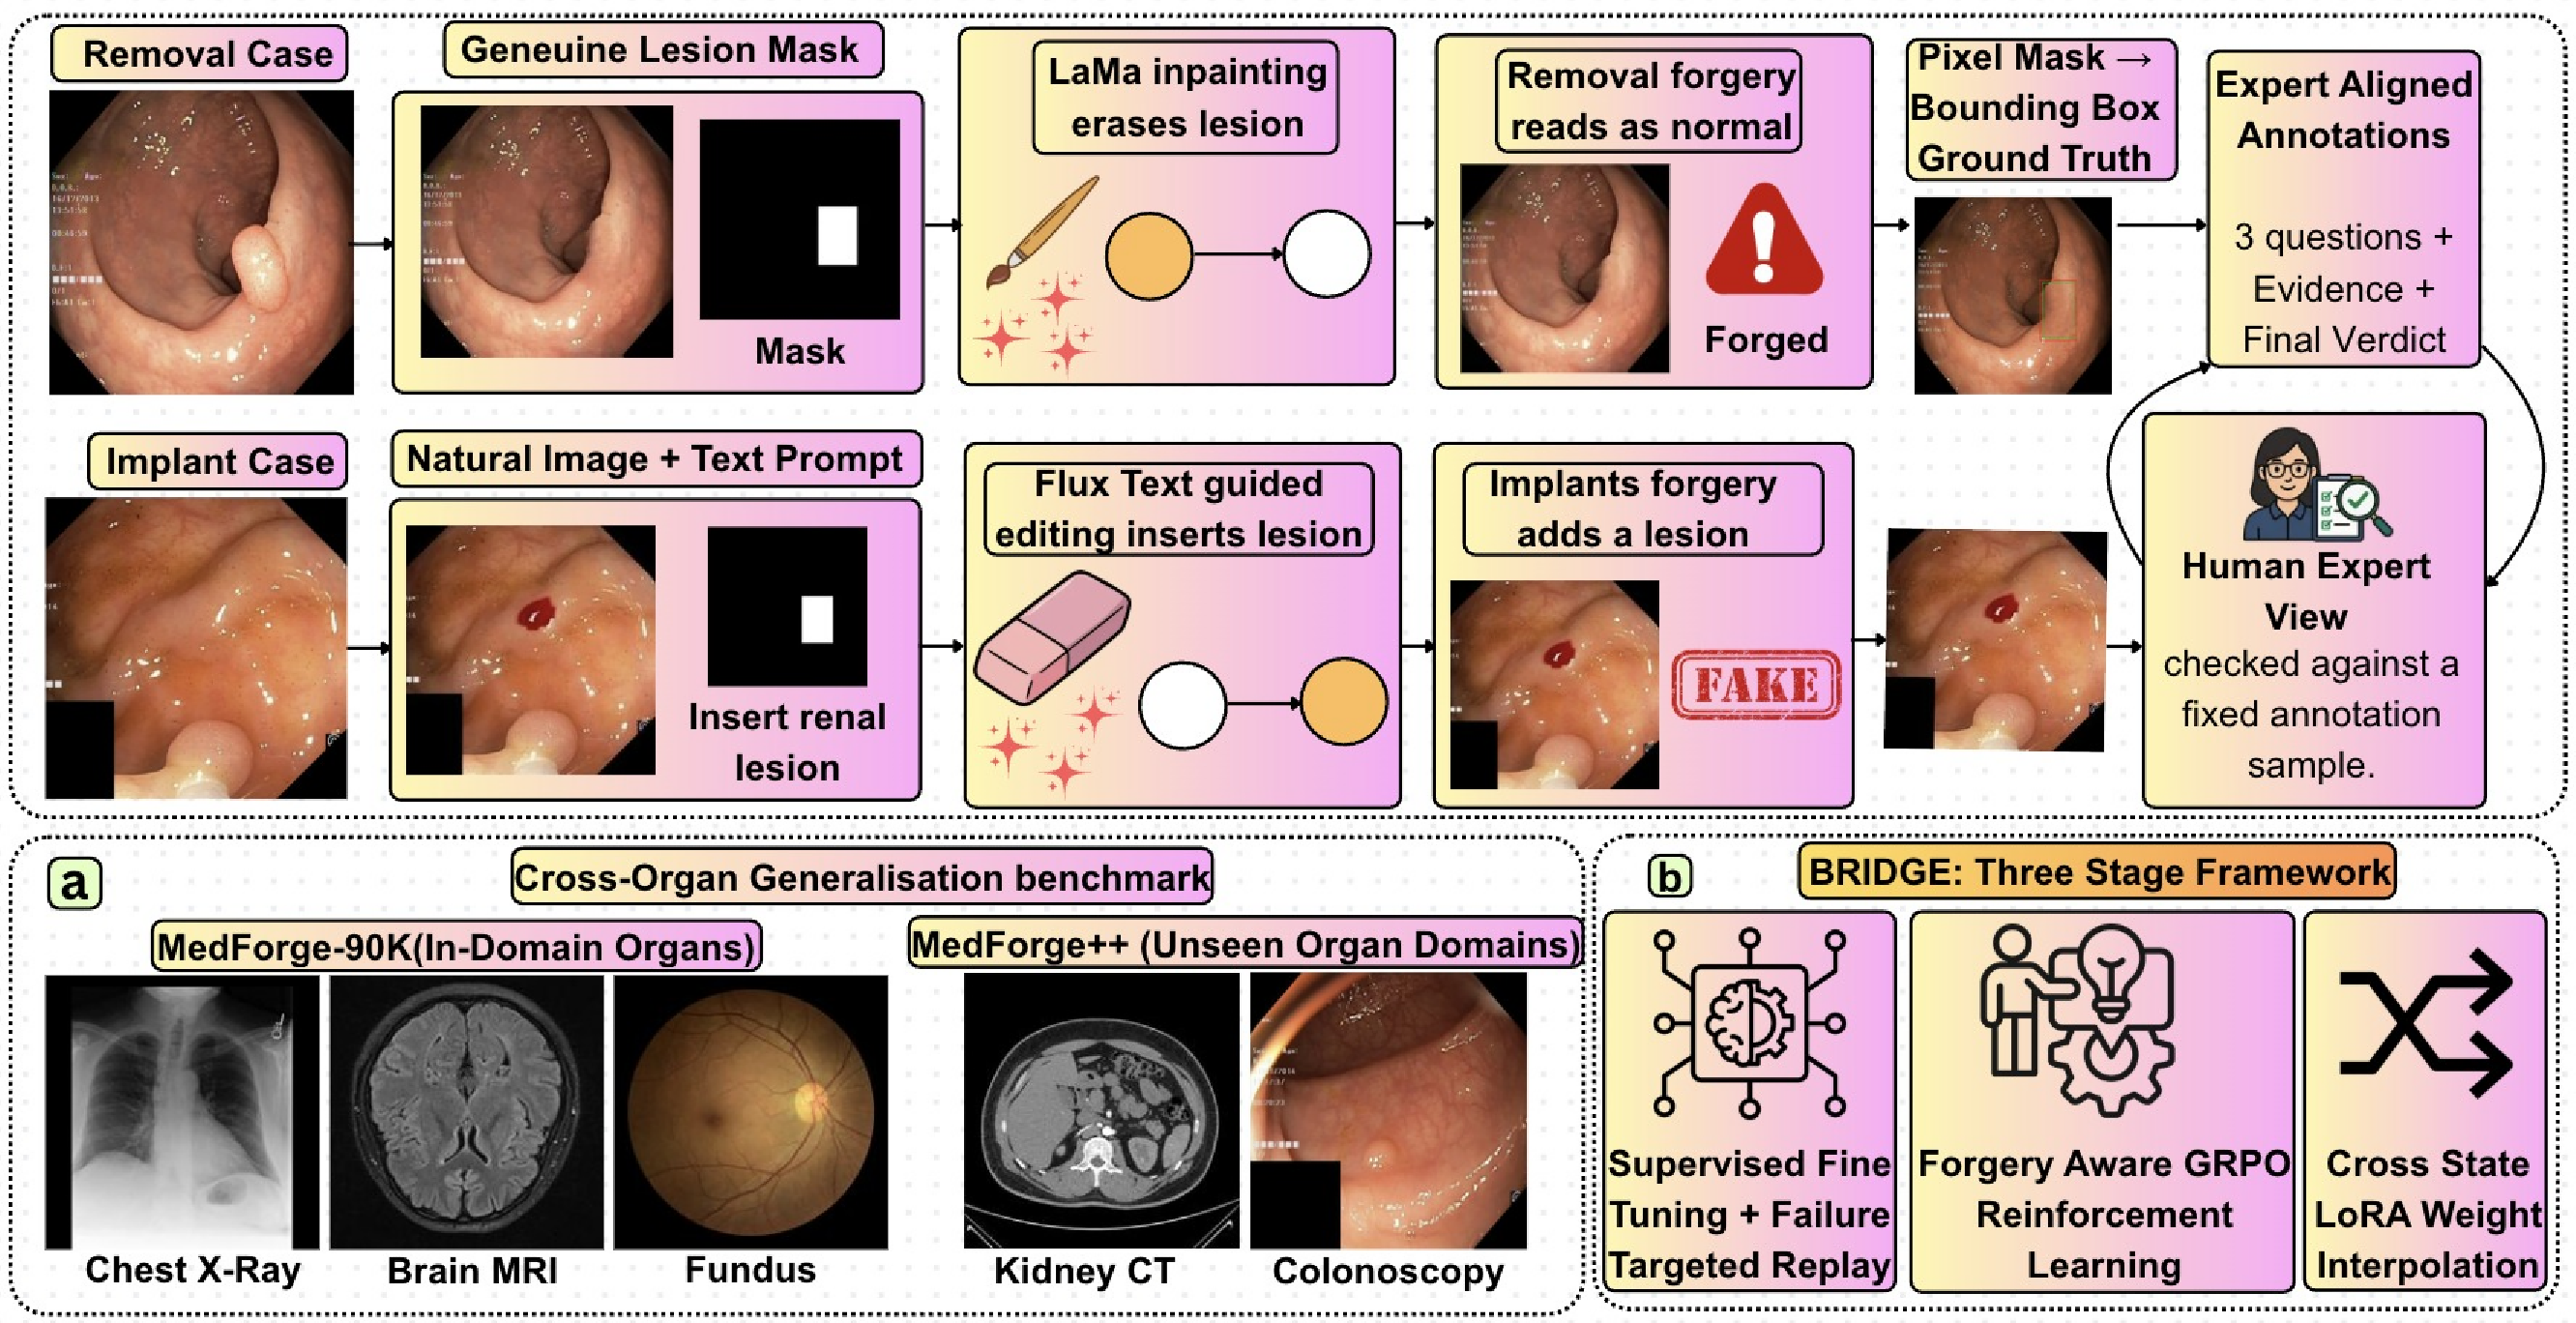
\includegraphics[width=\columnwidth]{figures/teaser_medforge++.pdf}
\caption{\textbf{(1)} \medforgepp{} dataset construction pipeline, \textbf{(2)} the cross-organ generalization benchmark, and \textbf{(3)} \bridge{}'s three-stage training framework (detailed in text).}
\label{fig:teaser}
\end{figure}

Detecting this kind of manipulation differs from natural-image deepfake detection: it is often a small regional edit in a noisy, modality-specific image with no face or identity to check, and the forensic cues are organ-specific, so detectors built for natural images transfer poorly \cite{medforge2026, natural_deepfake_survey_2024, biotampernet2026}. This holds even for the strongest natural-image detectors, whether they generalize across generators through frozen foundation features or up-sampling traces \cite{gan_fingerprint_detection_2020, clip_forgery_detection_2023, npr2024, fatformer2024} or localize splicing and inpainting artifacts at the pixel level \cite{trufor2023, hifinet2023}. Detection work has two families: black-box classifiers that output only a verdict, and reasoning-based detectors, increasingly multimodal LLMs trained with reinforcement learning, that localize and justify a verdict before committing \cite{medforge2026, vigil2026, grpo2024}, building on instruction-tuned and grounding-capable MLLMs \cite{llava15_2024, lisa2024} and on joint detection, localization, and explanation of natural-image deepfakes \cite{sida2025}. A separate literature studies why models fail under distribution shift across sites, scanners, and generators \cite{medical_domain_shift_2024, ood_generalization_survey_2024, fmsd2026, benchmark_diversity_2025}; Section~\ref{sec:related} surveys this, with an extended version in the Supplementary Material.

Together, these two threads leave a central gap. \medforge{}-90K, the largest annotated benchmark for this task, covers three organ families: chest X-ray, brain MRI, and fundus photography \cite{medforge2026}. Whether a detector trained on these generalizes to a fourth is untested, and this is not a minor extension: organs differ in tissue texture, anatomical variability, and imaging physics, so a boundary artifact diagnostic in one organ may be normal variation in another \cite{medical_domain_shift_2024, scanner_variability_2024}, and editing artifacts are themselves organ-specific: implanting a kidney tumor leaves different traces than erasing a colon polyp, even from the same editor \cite{lama2022}. A three-organ benchmark cannot tell us whether a detector learned organ-general reasoning or organ-specific shortcuts.

We address this gap by obtaining an officially released detector and testing it ourselves on new organs, rather than relying only on published in-distribution numbers. We extend \medforge{}-90K with \medforgepp{}, adding kidney CT and colon polyp images with both implant and removal forgeries in the same expert-aligned reasoning format, and introduce \bridge{}, a recipe combining supervised fine-tuning, reinforcement learning, and a lightweight model-merging step, evaluated under the same in-domain, cross-forgery, and cross-model protocols as prior work plus our new cross-organ setting. Figure~\ref{fig:teaser} illustrates this end to end: panel (1) shows the construction pipeline, where a Removal case erases a genuine lesion with LaMa inpainting and an Implant case inserts a synthetic lesion with a FLUX text-guided editor, both yielding a pixel mask converted to a bounding box that feeds an expert-aligned annotation (diagnostic questions, evidence, verdict); panel (2) contrasts \medforge{}-90K's in-domain organs (chest X-ray, brain MRI, fundus) with \medforgepp{}'s unseen organs (kidney CT, colonoscopy); and panel (3) shows \bridge{}'s three-stage framework, detailed in Section~\ref{sec:method}.

Our contributions are:
\begin{itemize}
\setlength{\itemsep}{1pt}
\setlength{\parskip}{0pt}
    \item \textbf{\medforgepp{}}, a multi-organ extension of \medforge{}-90K adding structured reasoning annotations for kidney CT and colon polyp forgeries, for 103{,}076 images total, enabling cross-organ evaluation for the first time here.
    \item \textbf{\bridge{}}, a Qwen3-VL-8B detector whose combined supervised and RL recipe sets a new state of the art on \medforge{}'s Cross-Forgery protocol on both accuracy and macro-F1.
    \item A \textbf{cross-organ evaluation} on \medforgepp{}'s new kidney and colon organs, where a dedicated \bridge{} $W_{\mathrm{SFT}}$ achieves 82.25\% accuracy, and a domain-routed deployment surpasses the released \medforge{}-Reasoner on the full multi-organ corpus.
\end{itemize}

\section{Related Work}
\label{sec:related}

\paragraph{Medical forgery generation and detection.} Generative editing has moved from GAN-based local manipulation to diffusion- and flow-based text-conditioned edits \cite{diffusion_survey_2024, latent_diffusion_2022, instruct_pix2pix_2023}. The CT-GAN attack showed as early as 2019 that a conditional GAN could inject or remove a lung nodule convincingly enough to fool radiologists \cite{ctgan_attack_2019}, and recent diffusion systems, datasets, and benchmarks generalize this across specialties \cite{medisyn_2024, miedb_2026, m3dsynth_2023, text_guided_medical_editing_2025, multimodal_foundation_models_2023, medical_data_augmentation_2023, gan_medical_synthesis_2022}. Detection has tracked these generators, from GAN-artifact detectors \cite{ctgan2022} to black-box classifiers with high in-distribution accuracy but no evidence, and reasoning-based detectors that localize and justify a verdict, most prominently the benchmark and detector for chest X-ray, brain MRI, and fundus photography \cite{medical_forgery_survey_2023, medforge2026}. Natural-image forgery detectors \cite{gan_fingerprint_detection_2020, vision_transformer_forgery_2023, clip_forgery_detection_2023, natural_deepfake_survey_2024} transfer poorly to organ- and modality-specific medical cues \cite{biotampernet2026}. No detector has been tested for whether its gains survive a shift to organs outside its training distribution, a gap this paper targets.

\paragraph{Explainable, reasoning-based detection and reinforcement learning.} Multimodal large language models suit the reason-then-verdict paradigm, since a single model can describe an image, pose diagnostic sub-questions, and only then commit to a classification \cite{qwenvl2024, qwen3vl2025}, and the current medical forgery state-of-the-art (SOTA) pairs localize-then-analyze inference with a forgery-aware alignment stage \cite{medforge2026}. Reinforcement learning (RL) has become the preferred way to align such reasoning models beyond supervised imitation, since a reward can encode properties of a good explanation difficult to specify through labeled examples alone \cite{ppo2017, grpo2024, rlhf_instructgpt_2022, chain_of_thought_2022}. Group-relative optimization and its sequence-level variant GSPO remove the need for a learned critic and align the current medical forgery SOTA \cite{grpo2024, gspo2025, medvlmr1_2025}. This is not risk-free: explanations can be post-hoc rather than grounded \cite{seeingbeforereasoning2025, vigil2026}, hallucinated reasoning is a documented VLM failure mode \cite{hallucination_vlm_2024, radiology_report_vlm_2023, medical_grounding_vlm_2024}, and reward hacking \cite{rewardhacking2026} is a closely related risk: a reward summing independent verdict, localization, and format terms lets a policy collect partial credit for a wrong verdict. The mere presence of an explanation also does not reliably raise clinician trust \cite{explainable_medical_ai_2025, clinical_trust_ai_2024}, and little work isolates which specific competency an RL stage actually improves \cite{reasoning_rl_visual_2024}.

\paragraph{Generalization and model merging.} Distribution shift across scanners, sites, and organs is a long-standing problem in medical imaging \cite{scanner_variability_2024, medical_domain_shift_2024, ood_generalization_survey_2024, domain_adaptation_medical_2023, federated_learning_medical_2023}, and cross-generator gaps are well documented in forgery detection, driven partly by narrow benchmark diversity \cite{fmsd2026, benchmark_diversity_2025, medical_benchmark_survey_2026, cross_organ_transfer_2024}. Separately, weight-space merging, model soups, task arithmetic, and their interference-reducing refinements \cite{modelsoups2022, task_arithmetic_2023, ties_merging_2023, dare_merging_2024, lorainterference2025, lora_orthogonal_merge_2025, modelinterp2025} combine models without extra training, but merging a supervised and a reinforcement-learning model trained on the \emph{same} task while specializing in different competencies remains unexplored. \bridge{} closes these gaps by extending evaluation to new organs, isolating the competency-specific effect of RL, and interpolating $W_{\mathrm{SFT}}$ and $W_{\mathrm{RL}}$ that share a training lineage.

\section{\medforgepp{} Dataset}
\label{sec:dataset}

Prior benchmarks for this task, most notably \medforge{}-90K, are built entirely from projection and 2D-based modalities: chest X-ray, brain MRI, and fundus photography \cite{medforge2026}. This leaves an important question unanswered: does a detector trained on these three organs learn forensic reasoning that generalizes to a genuinely different organ and modality, or does it learn shortcuts specific to the ones it was trained on? To probe this directly, we build \medforgepp{}, extending \medforge{}-90K with two organs chosen for their distance from the original three: kidney CT, a cross-sectional volumetric modality with tissue-texture statistics very different from projection radiography, and colonoscopy, an endoscopic video modality with no counterpart in \medforge{}-90K at all. Both are also clinically consequential targets for tampering, since a fabricated renal mass or a digitally erased colon polyp could each directly alter a diagnosis. \medforgepp{} combines the original \medforge{}-90K pool with 7{,}800 newly collected and annotated kidney-CT and colon-polyp images, for 103{,}076 images total (Table~\ref{tab:dataset}).

\begin{table}[t]
\centering
\small
\caption{\medforgepp{} composition. \medforge{}-90K figures are as reported by \citet{medforge2026}; the addition is this work.}
\label{tab:dataset}
\resizebox{\columnwidth}{!}{%
\begin{tabular}{lrrrr}
\toprule
Source & Real & Implant & Removal & Total \\
\midrule
\medforge{}-90K & 31{,}990 & 32{,}394 & 30{,}892 & 95{,}276 \\
\medforgepp{} addition & 3{,}800 & 2{,}000 & 2{,}000 & 7{,}800 \\
\midrule
\textbf{\medforgepp{} total} & \textbf{35{,}790} & \textbf{34{,}394} & \textbf{32{,}892} & \textbf{103{,}076} \\
\bottomrule
\end{tabular}%
}
\end{table}

\subsection{Organ and Subset Composition}
\label{sec:composition}
The addition spans two organs and eight labeled subsets, each 800--1{,}000 images (composition table in the Supplementary Material). Kidney images are axial, contrast-enhanced abdominal CT slices; colon images are colonoscopy video frames. Both differ substantially from \medforge{}-90K's three organs in acquisition geometry, tissue texture, and lesion presentation, which is why we use them to probe generalization rather than adding more images from a similar distribution. Subset-level results (Supplementary Material) show this gap is not uniform across the two organs.

\subsection{Forgery Pipeline}
\label{sec:pipeline}
The construction pipeline is summarized in Figure~\ref{fig:teaser}(1) and detailed in the Supplementary Material. Implant and removal forgeries use structurally different editing techniques, mirroring \medforge{}-90K's own implant/removal split so a Cross-Forgery protocol is directly comparable across the two datasets. Removal forgeries start from an authentic image with a genuine, radiologist-confirmed lesion; the lesion region is masked and erased with LaMa inpainting \cite{lama2022}, producing a scan that reads as normal but is not. Implant forgeries start from an authentic normal image and use a FLUX-based editor to insert a synthetic lesion at an anatomically plausible location, conditioned on a text description of the target pathology. Every forgery is paired with a pixel-level mask, from which we derive an axis-aligned bounding box as localization ground truth, consistent with \medforge{}-90K's box-based supervision. All images use a $1024\times1024$ canvas, matching \medforge{}-90K's coordinate convention.

\subsection{Expert-Aligned Reasoning Annotation}
\label{sec:annotation}
Following \medforge{}-90K's annotation philosophy, every training record pairs an image with a structured chain-of-thought target rather than a bare label. The target follows a forgery-type-aware self-questioning template with three diagnostic questions (boundary discontinuity, local texture consistency, and intensity plausibility), an evidence tag naming the dominant forensic cue, and a bounding box (or a ``no manipulated region identified'' token for authentic images), before the final verdict. Implant looks for a boundary artifact around an added structure; removal looks for over-smoothing where a structure was erased. We also built a second template that gives the localization decision before the verdict, and leave testing it as future work.

\section{Methodology}
\label{sec:method}

\bridge{} consists of three sequential training stages, shown in Figure~\ref{fig:bridge-arch}. Stage 1 pairs a medical image and text prompt with an expert-aligned annotation, fine-tunes the trainable Qwen3-VL-8B LM with a rank-32 LoRA adapter (vision encoder frozen) via cross-entropy SFT to obtain $W_{\mathrm{SFT}}$, mines held-out failures into a five-way \textsc{Solved}/\textsc{Localize}/\textsc{Verdict}/\textsc{Both}/\textsc{Hallucination.} Taxonomy, and continues LoRA SFT on the oversampled replay set to establish a strong classification baseline. Stage 2 samples $G{=}8$ diverse rollouts from $W_{\mathrm{SFT}}$, scores each with a classification-dominant reward $R(x,\hat y)$ gated on verdict correctness, computes the group-relative advantage $\hat A$, and updates the policy with the token-level PPO-clip objective $\mathcal{L}_{\mathrm{GRPO}}$ to obtain $W_{\mathrm{RL}}$, improving localization and reasoning quality. Stage 3 performs training-free interpolation between $W_{\mathrm{SFT}}$ and $W_{\mathrm{RL}}$ at a per-regime $\alpha$ (Eq.~\ref{eq:interp}), exploiting the bilinear cross-term of Eq.~\ref{eq:crossterm}, to produce \bridge{}'s final prediction: an authenticity classification, a manipulation localization, and an evidence-grounded explanation.

\begin{figure*}[t]
\centering
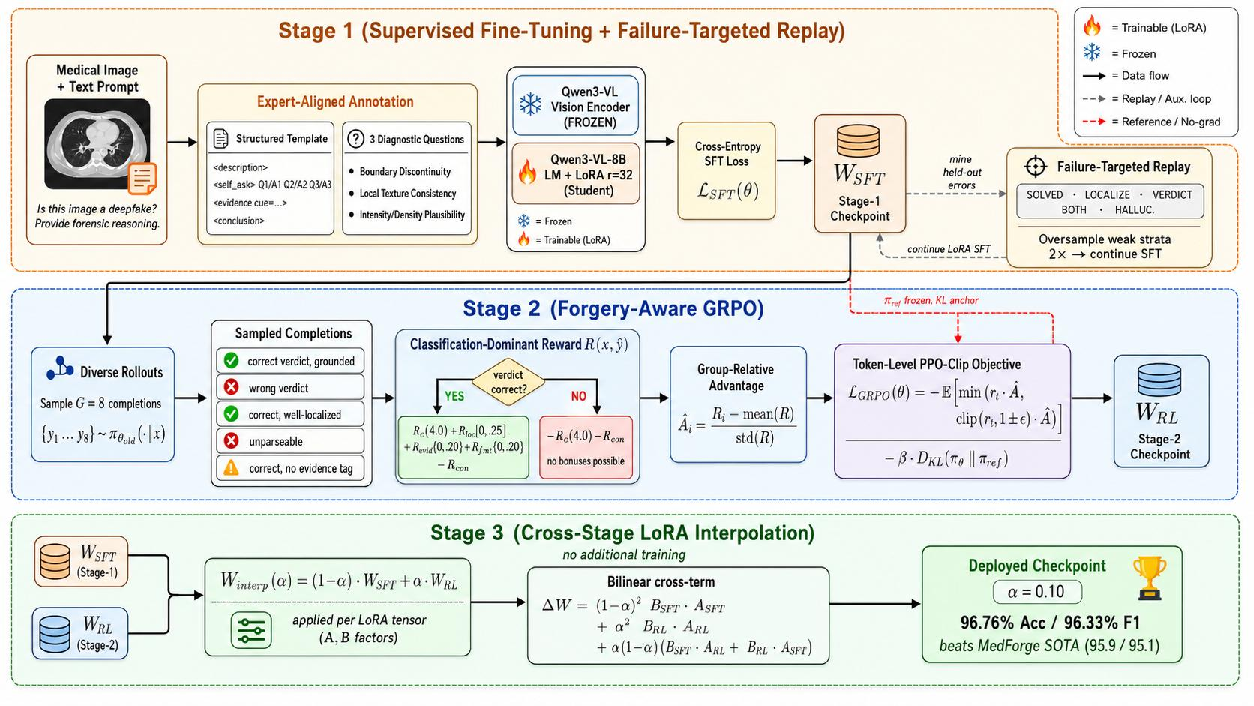
\includegraphics[width=0.84\textwidth]{figures/bridge.pdf}
\caption{\bridge{}'s three-stage architecture and training recipe: Stage 1 (failure-targeted replay SFT), Stage 2 (forgery-aware GRPO), and Stage 3 (cross-stage LoRA interpolation), producing \bridge{}'s final prediction.}
\label{fig:bridge-arch}
\end{figure*}

\subsection{Stage 1: Failure-Targeted Replay Supervised Fine-Tuning}
\label{sec:stage1}
Stage 1 begins with a medical image $x$ and a text prompt requesting a real-or-deepfake verdict. Each training pair aligns $x$ with an expert-aligned annotation $y$ (Section~\ref{sec:annotation}) that follows a structured template: a \texttt{<description>} field, a \texttt{<self\_ask>} block of three diagnostic question/answer pairs $Q_1$/$A_1$, $Q_2$/$A_2$, $Q_3$/$A_3$, an evidence tag, and a final \texttt{<conclusion>} giving the verdict $\hat v \in \{\text{real}, \text{deepfake}\}$ and, when applicable, a bounding box $\hat b$. The three diagnostic questions probe boundary discontinuity, local texture consistency, and intensity/density plausibility, the same forensic cues used to build \medforgepp{}'s annotations (Section~\ref{sec:pipeline}).

The policy $\pi_\theta$ is trained to reproduce $y$ from $x$. The Qwen3-VL vision encoder is kept frozen throughout this fine-tuning; only the language model, adapted with a rank-32 LoRA module \cite{lora2021}, is updated, so training shapes the reasoning and generation pathway without disturbing the visual features it conditions on. Fine-tuning uses the next-token cross-entropy objective,
\begin{equation}
\mathcal{L}_{\mathrm{SFT}}(\theta) = -\mathbb{E}_{(x,y)\sim\mathcal{D}}\sum_{t=1}^{T}\log P_\theta(y_t \mid x, y_{<t}).
\label{eq:sft}
\end{equation}
This first pass yields  $W_{\mathrm{SFT}}$. Uniform fine-tuning does not distinguish between examples the model already handles well and examples it consistently gets wrong. To target this, we mine $W_{\mathrm{SFT}}$'s held-out errors and introduce failure-targeted replay. The initial $W_{\mathrm{SFT}}$ is evaluated on a held-out split, and every prediction is assigned to one of five outcomes based on the ground-truth verdict $v$, the ground-truth box $b$ when one exists, the predicted verdict $\hat v$, and the predicted box $\hat b$. Here $\exists b$ denotes that a ground-truth manipulated region exists (a forged image), $\lnot\exists b$ that none exists (an authentic image), $\mathrm{IoU}(\hat b,b)$ the intersection-over-union between predicted and ground-truth boxes, and $\tau$ the IoU threshold for counting a box as well-localized:
\begin{equation}
f(x) = \begin{cases}
\textsc{Halluc.} & \lnot\exists b \wedge \hat b \ne \emptyset \\
\textsc{Solved} & \hat v = v \wedge (\lnot\exists b \vee \mathrm{IoU}(\hat b, b) \ge \tau) \\
\textsc{Localize} & \hat v = v \wedge \exists b \wedge \mathrm{IoU}(\hat b, b) < \tau \\
\textsc{Verdict} & \hat v \ne v \wedge (\lnot\exists b \vee \mathrm{IoU}(\hat b,b) \ge \tau) \\
\textsc{Both} & \hat v \ne v \wedge \exists b \wedge \mathrm{IoU}(\hat b,b) < \tau
\end{cases}
\label{eq:failure}
\end{equation}
with $\tau = 0.5$; cases are evaluated top to bottom and an empty or unparseable box counts as $\hat b = \emptyset$ (IoU $=0$). In words: \textsc{Solved} is a fully correct prediction (right verdict, and a well-localized box whenever one is expected); \textsc{Localize} is a correct verdict paired with a box that misses the ground truth; \textsc{Verdict} is a wrong verdict that is not accompanied by a poorly localized box; \textsc{Both} is a wrong verdict together with a poorly localized box; and \textsc{Halluc.} is a box emitted on an image where none should exist. This taxonomy separates verdict errors from localization errors and isolates hallucinated boxes, which lets replay target the specific failure mode of each example rather than treating every wrong prediction identically. Everything that is not \textsc{Solved} counts as an error; we group these errors into strata by manipulation type, organ, and pathology, then rank the strata by empirical failure rate. The weakest strata are oversampled at $2\times$ within a fixed budget and mixed with the remaining training pool, forming a replay set $\mathcal{D}_{\mathrm{replay}}$. A second round of LoRA fine-tuning continues from the $W_{\mathrm{SFT}}$ on $\mathcal{D}_{\mathrm{replay}}$, using the same objective (Eq.~\ref{eq:sft}). This replay-augmented model, denoted $W_{\mathrm{SFT}}$ for the remainder of the paper, is the strongest classifier among our models in this study (Section~\ref{sec:ablation}). Replay improves classification, but it does not directly optimize localization or reasoning quality, which motivates the reinforcement learning stage that follows.

\subsection{Stage 2: Reinforcement Learning with a Forgery-Aware Reward}
\label{sec:stage2}
Cross-entropy fine-tuning (Eq.~\ref{eq:sft}) rewards matching the reference text, not producing a well-localized, well-grounded verdict. Stage 2 addresses this by aligning $W_{\mathrm{SFT}}$ with reinforcement learning. For every prompt $x$, the policy generates a group of $G{=}8$ diverse rollouts, $\{y_i\}_{i=1}^G \sim \pi_{\theta_{\mathrm{old}}}(\cdot\mid x)$, spanning a range of outcomes (correct and evidence-grounded, wrong verdict, correct but poorly localized, unparseable, correct with no evidence tag). Each rollout is then scored by a classification-dominant reward, normalized into a group-relative advantage, and used to update the policy with a token-level clipped objective, as detailed below.

\paragraph{Classification-dominant reward.} The design of the reward $R(x,\hat y)$ determines what the policy is optimized to do. A common design sums independent terms for verdict correctness, localization, format, and evidence grounding, under which a wrong verdict can still collect substantial reward from the auxiliary terms. To prevent this, we gate the entire reward on verdict correctness: a completion earns its correctness reward and all applicable bonuses only if the verdict is right, and no bonuses otherwise. Formally,
\begin{equation}
R(x,\hat y) = \begin{cases}
\begin{aligned}[t]&R_{\mathrm{ver}} + R_{\mathrm{loc}} + R_{\mathrm{evid}}\\[-2pt] &\quad + R_{\mathrm{fmt}} - R_{\mathrm{con}}\end{aligned} & \hat v = v \\[6pt]
-R_{\mathrm{ver}} - R_{\mathrm{con}} & \hat v \ne v \\[2pt]
-R_{\mathrm{ver}} & \hat v \text{ unparseable}
\end{cases}
\label{eq:reward}
\end{equation}
with $R_{\mathrm{ver}} = 4.0$, $R_{\mathrm{loc}} = 0.25\cdot\mathrm{IoU}(\hat b, b) \in [0, 0.25]$ (zero if no ground-truth box), $R_{\mathrm{evid}} \in \{0, 0.20\}$ (paid if the reasoning names a forensic cue consistent with the manipulation type), $R_{\mathrm{fmt}} \in \{0, 0.20\}$ (paid for well-formed termination), and a contradiction penalty $R_{\mathrm{con}} = 1.0$ per internal inconsistency (a ``deepfake'' verdict with no box, or a ``real'' verdict with a non-empty box). Because $R_{\mathrm{loc}}$, $R_{\mathrm{evid}}$, and $R_{\mathrm{fmt}}$ are only added when $\hat v = v$, a well-localized, well-reasoned wrong answer cannot outscore a correct but plainly reasoned one.

\paragraph{Group-relative advantage.} Following Group Relative Policy Optimization \cite{grpo2024}, the group of rewards is normalized into a group-relative advantage $\hat A$,
\begin{equation}
\hat A_i = \frac{R(x,y_i) - \mathrm{mean}(\{R(x,y_j)\}_{j=1}^G)}{\mathrm{std}(\{R(x,y_j)\}_{j=1}^G) + \epsilon},
\label{eq:adv}
\end{equation}
which scores each rollout against its own group instead of relying on a learned value function; the constant $\epsilon$ prevents division by zero when a group's rewards are identical.

\paragraph{Token-level PPO-clip objective.} The policy is updated with a token-level PPO-style clipped objective \cite{ppo2017},
\begin{equation}
\resizebox{\columnwidth}{!}{$\displaystyle
\mathcal{L}_{\mathrm{GRPO}}(\theta) = -\mathbb{E}\Bigg[\frac{1}{G}\sum_{i=1}^{G}\frac{1}{|y_i|}\sum_{t=1}^{|y_i|} \min\!\Big(r_{i,t}(\theta)\hat A_i,\ \mathrm{clip}(r_{i,t}(\theta), 1{-}\varepsilon, 1{+}\varepsilon)\hat A_i\Big)\Bigg] + \beta\, D_{\mathrm{KL}}(\pi_\theta \Vert \pi_{\mathrm{ref}})
$}
\label{eq:grpo}
\end{equation}
where $r_{i,t}(\theta) = \pi_\theta(y_{i,t}\mid x, y_{i,<t}) / \pi_{\theta_{\mathrm{old}}}(y_{i,t}\mid x, y_{i,<t})$ is a \emph{token-level} importance ratio and $\pi_{\mathrm{ref}}$ is a frozen reference policy that anchors the KL term. In all reported runs $\beta{=}0$, i.e., no KL penalty is applied. The ratio is defined at the token level rather than the sequence level used by GSPO \cite{medforge2026}, which we found gives stable training in our setting. This stage produces the second output $W_{\mathrm{RL}}$, which specializes in localization while its classification accuracy remains close to $W_{\mathrm{SFT}}$; Section~\ref{sec:stage3} combines the two to recover both competencies at once.

\subsection{Stage 3: Cross-Stage LoRA Interpolation}
\label{sec:stage3}
Stage 3 combines $W_{\mathrm{SFT}}$ and $W_{\mathrm{RL}}$ through training-free weight interpolation, following prior work on model soups and reasoning checkpoints \cite{modelsoups2022,modelinterp2025}. Independently trained LoRA adapters can suffer interference from misaligned low-rank subspaces \cite{lorainterference2025}; ours share one training lineage because Stage 2 starts from Stage 1, so the checkpoints have identical tensor keys and shapes. This permits the direct blend
\begin{equation}
W_{\mathrm{interp}}(\alpha) = (1-\alpha)\, W_{\mathrm{SFT}} + \alpha\, W_{\mathrm{RL}}
\label{eq:interp}
\end{equation}
applied to every adapted layer's down- and up-projection factors $A$ and $B$. Since LoRA's effective update is bilinear, $\Delta W = BA$, interpolating the factors separately introduces a cross term,
\begin{equation}
\resizebox{\columnwidth}{!}{$\displaystyle
\Delta W_{\mathrm{interp}}(\alpha) = (1{-}\alpha)^2 B_{\mathrm{SFT}}A_{\mathrm{SFT}} + \alpha^2 B_{\mathrm{RL}}A_{\mathrm{RL}} + \alpha(1{-}\alpha)\big(B_{\mathrm{SFT}}A_{\mathrm{RL}} + B_{\mathrm{RL}}A_{\mathrm{SFT}}\big)
$}
\label{eq:crossterm}
\end{equation}
which is absent from either endpoint on its own. This cross term, acting on $W_{\mathrm{SFT}}$ and $W_{\mathrm{RL}}$, which make complementary errors, lets the interpolated model outperform \emph{both} endpoints rather than average them (Section~\ref{sec:ablation}). In practice, $\alpha$ is selected per regime by sweeping a fixed grid, $\alpha \in \{0.00, 0.05, \ldots, 0.40\}$, and deploying whichever value jointly maximizes accuracy and macro-F1 (Table~\ref{tab:ablation-interp}). Interpolation is best on Cross-Forgery and In-Domain, but not Cross-Model, where $W_{\mathrm{RL}}$ alone is deployed. Together, the three stages implement a division of labor: Stage 1 anchors classification, Stage 2 specializes in localization, and Stage 3 combines both at no additional training cost.

At inference, the deployed model produces a single structured output with three named components, shown as \bridge{}'s final prediction in Figure~\ref{fig:bridge-arch}: an \emph{authenticity classification} ($\hat v$, the real-or-deepfake verdict), a \emph{manipulation localization} ($\hat b$, the bounding box on the manipulated region when one is predicted), and an \emph{evidence-grounded explanation} (the structured reasoning trace and evidence tag that justify $\hat v$ and $\hat b$). These three components are exactly the sequence $y$ defined at the start of this section; Stage 3 changes only which model's weights produce them, not their structure.

\section{Experiments}
\label{sec:exp}

\subsection{Experimental Setup}
\label{sec:setup}
We adopt the 5:1:3 split of \medforge{}~\cite{medforge2026} on \medforge{}-90K (training pool / held-out pool; the 95{,}276 images include 5{,}276 beyond the nominal 90K, and the Stage-2 rollout prompts are drawn from the same training pool as Stage 1), drawing a shared, stratified 2{,}994-image test set (994 real / 1{,}000 implant / 1{,}000 removal) used across all regimes, plus an 800-image held-out \medforgepp{} split for cross-organ generalization. We evaluate under three regimes, defined by what is withheld from training: \emph{In-Domain} (nothing withheld), \emph{Cross-Forgery} (implant manipulations withheld), and \emph{Cross-Model} (four advanced generator models withheld). All \bridge{} models are Qwen3-VL-8B with a rank-32 LoRA adapter; Stage-1 SFT uses learning rate $10^{-5}$, Stage-2 GRPO uses $10^{-6}$ with group size $G{=}8$ and $\beta{=}0$. We report accuracy, macro-F1, mIoU, and IoU@0.5 with the same harness for every model, including the released \medforge{}-Reasoner, evaluated with its own documented prompt and token budget after correcting a verdict-parser artifact (Supplementary Material).

\subsection{Main Results}
\label{sec:main}
Table~\ref{tab:main} reports \bridge{} against \medforge{} existing methods across all three regimes, using the same per-class-averaged macro-F1 convention so the two are directly comparable. On \emph{Cross-Forgery}, \bridge{} reaches 96.96\%/96.18\% accuracy/F1, a new state of the art over \medforge{}'s published 95.93\%/95.13\%. On \emph{Cross-Model}, \bridge{} reaches 94.66\%/94.62\%, ahead of \medforge{}'s published 93.94\%/93.49\%. On \emph{In-Domain}, \bridge{} reaches 99.03\%/98.87\%, close to but just under \medforge{}'s published 99.23\%/98.98\%, an already near-ceiling regime. Which stage of our recipe supplies the deployed model differs by regime; Section~\ref{sec:ablation} breaks this down.

\begin{table}[t]
\centering
\small
\caption{\bridge{} versus \medforge{}~\cite{medforge2026}, test $n{=}2{,}994$. Each regime reports the best of the three \bridge{} stages (Section~\ref{sec:ablation}): Cross-Forgery/In-Domain select $\alpha{=}0.15$ interpolation; Cross-Model selects Stage-2 GRPO directly. Macro-F1 is the per-class one-vs-rest average, matching \medforge{}'s convention. The released \medforge{}-Reasoner checkpoint scores 99.83/99.81 on this test set when re-evaluated with our harness; since its training split is unknown and may overlap our test images, we treat that number as an upper bound rather than a comparable result.}
\label{tab:main}
\resizebox{\columnwidth}{!}{%
\begin{tabular}{lrrrrrr}
\toprule
& \multicolumn{2}{c}{In-Domain} & \multicolumn{2}{c}{X-Forgery} & \multicolumn{2}{c}{X-Model} \\
Model & Acc. & F1 & Acc. & F1 & Acc. & F1 \\
\midrule
\medforge{}~\cite{medforge2026} & \textbf{99.23} & \textbf{98.98} & 95.93 & 95.13 & 93.94 & 93.49 \\
\textbf{\bridge{} (ours)} & 99.03 & 98.87 & \textbf{96.96} & \textbf{96.18} & \textbf{94.66} & \textbf{94.62} \\
\bottomrule
\end{tabular}%
}
\end{table}

\subsection{Detailed Per-Class Comparison}
\label{sec:perclass}
Table~\ref{tab:published-full} compares \bridge{} against \medforge{}'s published per-class results \cite{medforge2026} -- specialized detectors, generic MLLM baselines, and \medforge{}-Reasoner -- broken down by class (Real, Implant, Remove) and regime. Cross-Forgery and In-Domain use the $\alpha{=}0.15$ interpolation (Stage 3); Cross-Model uses $W_{\mathrm{RL}}$ (Section~\ref{sec:ablation}). \bridge{} exceeds \medforge{}-Reasoner's published Cross-Model and Cross-Forgery averages on both accuracy and F1, and is within 0.20/0.11 points on In-Domain.

\begin{table*}[t]
\centering
\resizebox{\textwidth}{!}{%
\begin{tabular}{lcccccccccccc}
\toprule
\multirow{2}{*}{Method} & \multicolumn{3}{c|}{Real} & \multicolumn{3}{c|}{Forgery: Implant} & \multicolumn{3}{c|}{Forgery: Remove} & \multicolumn{3}{c}{Average} \\
 & In-Dom.\ & X-Forg.\ & X-Model & In-Dom.\ & X-Forg.\ & X-Model & In-Dom.\ & X-Forg.\ & X-Model & In-Dom.\ & X-Forg.\ & X-Model \\
\midrule
\multicolumn{13}{c}{\textit{Accuracy (\%), published~\cite{medforge2026}}} \\
\midrule
SIDA-7B~\cite{sida2025} & 77.56 & 73.14 & 73.42 & 79.83 & 76.18 & 76.57 & 82.31 & 77.92 & 75.68 & 79.90 & 75.75 & 75.22 \\
SIDA-13B~\cite{sida2025} & 89.37 & 85.68 & 84.25 & 91.52 & 87.24 & 85.86 & 93.84 & 90.17 & 86.53 & 91.58 & 87.70 & 85.55 \\
FakeVLM & 86.48 & 81.86 & 76.94 & 88.93 & 83.57 & 79.82 & 91.27 & 86.35 & 82.51 & 88.89 & 83.93 & 79.76 \\
AIGI-Holmes & 90.24 & 86.53 & 84.37 & 88.12 & 84.46 & 80.91 & 90.58 & 90.64 & 87.23 & 89.65 & 87.21 & 84.17 \\
Qwen3-VL-Flash & 57.60 & 55.50 & 54.90 & 47.83 & 50.47 & 50.93 & 54.17 & 54.17 & 54.61 & 53.20 & 53.38 & 53.48 \\
Qwen3-VL-Plus & 54.14 & 54.28 & 55.10 & 57.42 & 55.78 & 56.03 & 55.80 & 55.86 & 56.10 & 55.79 & 55.31 & 55.74 \\
Gemini 3 Flash & 71.26 & 73.39 & 72.57 & 57.33 & 62.46 & 60.14 & 57.14 & 62.27 & 60.34 & 61.91 & 66.04 & 64.35 \\
Gemini 3 Pro & 67.29 & 65.11 & 64.49 & 75.34 & 75.24 & 74.80 & 65.05 & 66.49 & 65.70 & 69.23 & 68.95 & 68.33 \\
\medforge{}-Reasoner & \textbf{99.24} & \textbf{95.24} & 92.86 & 99.24 & 93.39 & \textbf{94.86} & \textbf{99.21} & \textbf{99.15} & \textbf{94.09} & \textbf{99.23} & 95.93 & 93.94 \\
\textbf{\bridge{} (ours)} & 98.99 & 95.17 & \textbf{99.40} & \textbf{99.60} & \textbf{97.10} & 91.90 & 98.50 & 98.60 & 91.80 & 99.03 & \textbf{96.96} & \textbf{94.66} \\
\midrule
\multicolumn{13}{c}{\textit{F1 Score (\%), published~\cite{medforge2026}}} \\
\midrule
SIDA-7B~\cite{sida2025} & 76.84 & 72.47 & 67.73 & 86.47 & 74.06 & 69.85 & 81.64 & 77.28 & 72.94 & 81.65 & 74.60 & 70.17 \\
SIDA-13B~\cite{sida2025} & 88.69 & 84.95 & 80.58 & 90.86 & 86.57 & 83.17 & 93.18 & 89.46 & 85.87 & 90.91 & 86.99 & 83.21 \\
FakeVLM & 85.73 & 81.18 & 76.29 & 88.27 & 82.86 & 79.16 & 90.58 & 85.67 & 81.84 & 88.19 & 83.24 & 79.10 \\
AIGI-Holmes & 88.57 & 85.84 & 86.68 & 90.46 & 88.73 & 84.25 & 89.82 & 85.97 & 83.58 & 89.62 & 86.85 & 84.84 \\
Qwen3-VL-Flash & 32.48 & 38.62 & 40.26 & 55.08 & 53.70 & 52.69 & 63.13 & 59.51 & 58.78 & 50.23 & 50.61 & 50.58 \\
Qwen3-VL-Plus & 47.73 & 46.36 & 46.18 & 54.70 & 53.91 & 54.99 & 52.42 & 54.26 & 55.32 & 51.62 & 51.51 & 52.16 \\
Gemini 3 Flash & 24.42 & 41.14 & 34.78 & 70.22 & 72.05 & 71.11 & 70.07 & 71.91 & 71.34 & 54.90 & 61.70 & 59.08 \\
Gemini 3 Pro & 61.82 & 62.64 & 62.22 & 74.22 & 71.53 & 71.02 & 59.47 & 57.62 & 56.19 & 65.17 & 63.93 & 63.14 \\
\medforge{}-Reasoner & \textbf{98.86} & 93.29 & 92.07 & 98.86 & 92.97 & 94.63 & \textbf{99.21} & \textbf{99.14} & 93.76 & \textbf{98.98} & 95.13 & 93.49 \\
\textbf{\bridge{} (ours)} & 98.55 & \textbf{95.41} & \textbf{92.12} & \textbf{99.30} & \textbf{96.19} & \textbf{95.48} & 98.75 & 96.95 & \textbf{95.43} & 98.87 & \textbf{96.18} & \textbf{94.62} \\
\bottomrule
\end{tabular}%
}
\caption{Per-class results on \medforge{}-90K: published baselines from \citet{medforge2026} (SIDA, FakeVLM, AIGI-Holmes, generic MLLMs, \medforge{}-Reasoner), plus \bridge{} (ours). Cross-Forgery and In-Domain use the $\alpha{=}0.15$ interpolation (Stage 3); Cross-Model uses the Stage-2 GRPO model $W_{\mathrm{RL}}$ directly, the best of the three stages for that regime. Bold marks the higher of \medforge{}-Reasoner and \bridge{} (ours) per column.}
\label{tab:published-full}
\end{table*}

\subsection{Results on \medforgepp{}: Cross-Organ Generalization}
\label{sec:mfpp}

\begin{table}[t]
\centering
\small
\begin{tabular}{lrr}
\toprule
Class & Recall & F1 \\
\midrule
Real & 95.25 & 84.29 \\
Implant & 99.50 & 95.22 \\
Remove & 39.00 & 52.53 \\
\midrule
\textbf{Average} & \textbf{82.25} & \textbf{77.34} \\
\bottomrule
\end{tabular}
\caption{\bridge{} on \medforgepp{} (kidney CT / colon polyp), $W_{\mathrm{SFT}}$ (dedicated \medforgepp{} SFT). \medforgepp{} is evaluated as a single held-out split rather than \medforge{}'s three-tier protocol, so only one column is reported. The Remove class is the dominant failure mode, consistent with the per-subset breakdown in the Supplementary Material.}
\label{tab:bridge-medforgepp}
\end{table}

On \medforgepp{}'s 800-image kidney/colon held-out split (Table~\ref{tab:bridge-medforgepp}), a dedicated \bridge{} $W_{\mathrm{SFT}}$ trained directly on \medforgepp{} reaches \textbf{82.25\% accuracy and 77.34\% macro-F1} on this new-organ split. On the complete \medforgepp{} distribution, a $3{,}794$-image aggregate test set (2{,}994 \medforge{} organs + 800 kidney/colon) drawn from the 103{,}076-image corpus, our recipe produces domain-specialized models that share an evaluation interface, so an organ-routed deployment of \bridge{} (selecting the specialist per image) reaches \textbf{93.86\% accuracy and 93.49\% macro-F1} (Table~\ref{tab:medforgepp-agg}), surpassing the released \medforge{}-Reasoner's \textbf{89.85\%/89.05\%} by 4.01/4.44 points, with the imaged organ known at inference time.

\begin{table}[t]
\centering
\small
\caption{\bridge{} versus the released \medforge{}-Reasoner on the 3{,}794-image \medforgepp{} aggregate test set spanning all five organs (organ-routed; the imaged organ is assumed known). Both are evaluated with the same harness.}
\label{tab:medforgepp-agg}
\begin{tabular}{lrr}
\toprule
Model & Acc. & Macro-F1 \\
\midrule
\medforge{}-Reasoner (released) & 89.85 & 89.05 \\
\textbf{\bridge{} (ours)} & \textbf{93.86} & \textbf{93.49} \\
\bottomrule
\end{tabular}
\end{table}

\subsection{Reasoning Quality}
\label{sec:reasoning}
As a verifiable proxy for reasoning quality we report format well-formedness: parse-verdict rate is $\ge 99.97\%$ and parse-box rate is 67--75\% across every \bridge{} model in Table~\ref{tab:main}. The near-perfect parse-verdict rate means \bridge{}'s outputs are almost always machine-readable, a prerequisite for automated triage, and the parse-box rate is consistent with the roughly one-third of test images that are authentic and correctly emit no box. A qualitative walkthrough of held-out examples is given in the Supplementary Material.

\subsection{Ablation Studies}
\label{sec:ablation}
\paragraph{Complementary specialization of the RL stage.} Across every Stage-2 configuration we trained (varying reward design, $\beta$, and step budget; full table in the Supplementary Material), forgery-aware RL consistently lifts localization: every configuration that includes a localization term reaches an mIoU at or above Stage 1's 24.06, with the best reaching 28.84, while classification accuracy stays anchored by the supervised replay stage. This clean separation is precisely what makes $W_{\mathrm{SFT}}$ and $W_{\mathrm{RL}}$ productive to interpolate. A per-term reward ablation (Supplementary Material) confirms no single bonus is redundant: removing $R_{\mathrm{loc}}$ hurts mIoU most, removing $R_{\mathrm{evid}}$ hurts accuracy and F1 most, and removing $R_{\mathrm{fmt}}$ falls between the two. A further ablation isolating single competencies (Supplementary Material) finds a localization-only reward reaches the highest accuracy of any Stage-2 configuration (95.46) but the lowest mIoU (23.32), the reverse of the expected pattern, suggesting Stage 1's classification behavior survives GRPO regardless of what the reward targets, while box-emission specifically depends on localization being part of the signal.

\paragraph{Interpolation ratio.} We sweep $\alpha \in \{0.00, \ldots, 0.40\}$ in steps of 0.05 between the replay-SFT and the top-performing RL model $W_{\mathrm{RL}}$ (full sweep in the Supplementary Material). Table~\ref{tab:ablation-interp} shows the pattern: accuracy and F1 both peak at $\alpha{=}0.15$, then decline monotonically through $\alpha{=}0.40$, while mIoU increases roughly monotonically with $\alpha$ throughout. We deploy $\alpha{=}0.15$ since it maximizes both accuracy and F1 at once; none of these values transfers this advantage to \medforgepp{} (Section~\ref{sec:mfpp}).

\begin{table}[t]
\centering
\small
\caption{Interpolation ratio ablation (Eq.~\ref{eq:interp}), Cross-Forgery test set; full 0.05-step sweep in the Supplementary Material.}
\label{tab:ablation-interp}
\begin{tabular}{lrrr}
\toprule
$\alpha$ & Acc.\ & F1 & mIoU \\
\midrule
0.00 (SFT endpoint) & 95.76 & 94.16 & 24.06 \\
0.15 (deployed) & \textbf{96.96} & \textbf{96.18} & 24.70 \\
0.40 & 96.19 & 95.19 & \textbf{26.29} \\
\bottomrule
\end{tabular}
\end{table}

\paragraph{Why interpolation helps: error complementarity.} Cross-tabulating the verdicts of $W_{\mathrm{SFT}}$ and $W_{\mathrm{RL}}$ on the Cross-Forgery test set (Table~\ref{tab:overlap}), they disagree on 4.31\% of images, split almost evenly between cases only Stage 1 gets right (2.40\%) and only Stage 2 gets right (1.90\%): their errors are complementary, not redundant. An oracle selecting the correct model per image would reach 97.66\%; the interpolated model at $\alpha{=}0.15$ realizes 96.96\%, capturing 63\% of that headroom with no additional training, consistent with the cross-term analysis of Section~\ref{sec:stage3}. A per-class breakdown (Supplementary Material) shows this complementarity is concentrated on Real images (83.80\% agreement, versus 97.60\%/98.60\% on Implant/Remove): the gain is driven by disagreements over whether an image was manipulated at all, not over forgery type.

\begin{table}[t]
\centering
\small
\caption{Per-sample verdict agreement between the Stage-1 (replay-SFT) and Stage-2 (best RL) models, Cross-Forgery test set ($n{=}2{,}994$). Their complementary errors are what interpolation exploits.}
\label{tab:overlap}
\begin{tabular}{lr}
\toprule
Outcome & \% of test set \\
\midrule
Both correct & 93.35 \\
Only Stage 1 (SFT) correct & 2.40 \\
Only Stage 2 (RL) correct & 1.90 \\
Both wrong & 2.34 \\
\midrule
Oracle (either correct) & 97.66 \\
Interpolation $\alpha{=}0.15$ (realized) & 96.96 \\
\bottomrule
\end{tabular}
\end{table}

\paragraph{Interpolation benefit is regime-specific.} The regimes diverge (Table~\ref{tab:main}): In-Domain follows the Cross-Forgery pattern (interpolation best), while on Cross-Model $W_{\mathrm{RL}}$ alone remains best. The complementary-errors mechanism of Section~\ref{sec:stage3} thus benefits two of the three regimes, a regime-specific rather than organ-specific property.

\section{Conclusion}
\label{sec:conclusion}
We introduced \medforgepp{}, a multi-organ extension of \medforge{}-90K, and \bridge{}, a three-stage detector combining failure-targeted replay SFT, a classification-dominant forgery-aware GRPO reward, and cross-stage LoRA weight interpolation. Our central finding is a division of labor: supervised replay anchors classification, RL specializes in localization, and a training-free interpolation of the two surpasses either endpoint, setting a new state of the art on Cross-Forgery (96.96\%/96.18\% vs.\ 95.93\%/95.13\%). On the new organs of \medforgepp{}, a dedicated \bridge{} $W_{\mathrm{SFT}}$ reaches 82.25\% accuracy, and a domain-routed deployment reaches 93.86\%/93.49\% aggregate accuracy/macro-F1 on the full multi-organ corpus, surpassing the released \medforge{}-Reasoner's 89.85\%/89.05\%. We release \medforgepp{}, our tooling, and reward and interpolation implementations to support future work in trustworthy medical image forensics.

{
    \small
    \bibliographystyle{ieeenat_fullname}
    \bibliography{references}
}

\end{document}
